\chapter{Marco teórico}

\section{Metodología de validación de videojuegos educativos}

Petri y Gresse von Wangenheim, en su trabajo \cite{HowGamesComputingEducationEvaluated}, llevaron a cabo una revisión de la literatura antes de desarrollar el modelo MEEGA+, cuya publicación tuvo lugar en 2018 \cite{meegaplus}. En dicha revisión, analizaron la evaluación de videojuegos educativos relacionados con la computación a partir de una muestra de 3617 artículos. Clasificaron los estudios según la metodología empleada en verdaderos estudios, cuasi-experimentales, no experimentales y ad-hoc.

Los estudios que distribuían personas de forma aleatoria en distintos grupos se consideraron experimentales. Si un estudio emplea múltiples grupos o momentos de medida sin asignación aleatoria, se clasificaba como cuasi-experimental. Los estudios que no utilizaban múltiples grupos, pero que se llevaban a cabo de manera sistemática con estudios de casos, se consideraban no experimentales. Por último, los estudios que no se llevaban a cabo de manera sistemática, ni indican cómo se miden resultados, se clasificaban como estudios ad-hoc.

En una reseña de literatura realizada por Calderón y Ruiz \cite{CalderonRuizReviewSeriousGamesEvaluation} destacaron que la mayoría de los estudios sobre videojuegos educativos se centran en la evaluación del aprendizaje, la usabilidad y la experiencia del usuario. Además, observaron que la mayoría de estos estudios se llevan a cabo de manera ad-hoc, sin una sistematización adecuada. Se evidenció que los métodos de validación más comunes son cuestionarios y entrevistas. Asimismo, en su trabajo se propuso una categorización de características que indican la calidad de un juego, la cual fue posteriormente utilizada por los autores de MEEGA+ \cite{meegaplus} en su cuestionario. Entre los aspectos evaluados se incluyen: el diseño del juego, la satisfacción del usuario, la usabilidad, la motivación y los resultados del aprendizaje, entre otros.

En su revisión sobre videojuegos serios, Calderón y Ruiz \cite{CalderonRuizReviewSeriousGamesEvaluation} también categorizaron los métodos utilizados para validar estos trabajos en tres tipos: simple, pre/post y pre/post/post. En el primer enfoque, se llevaba a cabo una sesión de juego y luego se aplicaban los mecanismos de evaluación. En el segundo, se realizaban evaluaciones antes y después del juego para medir el conocimiento previo y adquirido. En el tercero, además de las evaluaciones pre y post, se llevaba a cabo una prueba semanas después para evaluar la retención. En cuanto a las frecuencias, 50 de 89 de estos estudios utilizaron una metodología simple y el 55\% lo hizo con tamaños de muestra inferiores a 40 \cite{CalderonRuizReviewSeriousGamesEvaluation}.

Basándose en estas conclusiones, Petri y Christiane Gresse von Wangenheim, en su revisión de literatura sobre videojuegos educativos \cite{HowGamesComputingEducationEvaluated}, afirman que la mayoría de los estudios sobre videojuegos educativos se realizan de manera ad-hoc en términos de diseño de investigación, medición, recolección de datos y análisis. Sin embargo, destacan el modelo MEEGA+ \cite{meegaplusQualityEvaluationPage}, indicando que ha sido utilizado en otras áreas distintas de la computación, proporcionando mayor sistematización y confiriendo mayor validez científica a los trabajos basados en este modelo.

\section{Teoría de Respuesta al Ítem (IRT): Intuición Cualitativa}

La Teoría de Respuesta al Ítem (IRT) es un modelo estadístico utilizado en pruebas globales, como exámenes de inglés como lengua extranjera y programas de evaluación internacional de estudiantes. Este modelo destaca por su capacidad para evaluar detalladamente propiedades estadísticas de cada ítem (o pregunta) en términos de dificultad y capacidad de diferenciación \cite{Linden2015HandbookOI, IRTShojima2022}.

Los modelos basados en IRT parten de tres suposiciones fundamentales. Primero, establecen una relación entre el rasgo latente que se busca medir y la probabilidad de responder un ítem en una categoría específica, como ``en desacuerdo'' o ``de acuerdo'' \cite{CalderonStatisticalIRT}.

El segundo supuesto es que existe una escala continua y unidimensional de habilidad, denotada como $\theta$. Aunque esta suposición es fuerte, hay técnicas para verificar la unidimensionalidad de los datos de prueba \cite{IRTShojima2022}. Para medir múltiples características simultáneamente, existen modelos IRT multidimensionales \cite{Reckase2009MultidimensionalIRT}.

La tercera suposición es la independencia local, que establece que las personas responden de forma independiente a cada ítem o pregunta, sin que la respuesta a una influya en la respuesta a otra \cite{CalderonStatisticalIRT}.

Por definición, $\theta$ está en el rango $]-\infty, \infty [$, pero prácticamente la totalidad de los datos está en el rango aproximado de $]-3, 3[$. Un valor $\theta = 0$ se asume como un nivel promedio \cite{IRTShojima2022}. 

El modelo de 2 parámetros (2PLM o Two-Parameter Logistic Model) considera la dificultad y la discriminación (difficulty \& discrimination) de cada ítem. La dificultad se refiere a qué tan difícil es un ítem en relación con otros; mientras que la discriminación se refiere a la capacidad del ítem para distinguir entre participantes con diferentes niveles de habilidad. 

Existen distintos modelos logísticos para evaluar $\theta$. El que se usa en este trabajo es el modelo logístico de 2 parámetros y otra variante de tres parámetros. Los parámetros en estos casos buscan representar rasgos asociados a cada ítem o pregunta. El de 2 parámetros incluye dificultad y discriminación, aunque en español se podría interpretar mejor como distinción o graduación, asociado a indicar la probabilidad entre elegir un valor u otro \cite{CalderonStatisticalIRT}.  El valor de $\theta$ se puede aproximar utilizando el método bayesiano EAP (Expected A Posteriori), el cual se calcula utilizando los paquetes de R \textit{mirt} \cite{RMIRT} y \textit{mirtCAT} \cite{RPackageMIRTCAT} aplicados en este trabajo. 

El modelo 2PLM se compone del parámetro dificultad $b_j$ y de discriminación $a_j$ asignados para cada pregunta. Este último representa la pendiente de la curva e indica en qué medida el ítem diferencia a los examinados con un nivel en el rasgo latente por encima o debajo del parámetro de dificultad \cite{TeoriaRespuestaAlItemPsicologia}. En un modelo con respuestas correctas e incorrectas, un ítem con un parámetro de dificultad mayor $b_j$ será respondido incorrectamente con mayor probabilidad para casi cualquier nivel de $\theta$ \cite{IRTShojima2022}.


\begin{figure}[h]
	\centering
	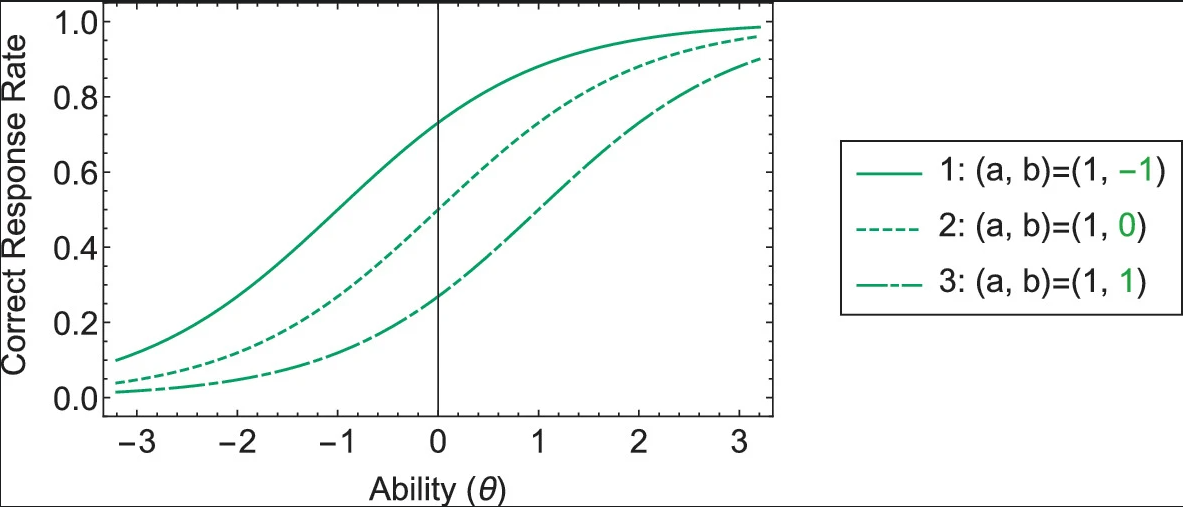
\includegraphics[scale=.5]{imagenes/IRTparambdifficulty.png}
	\caption{Probabilidad de responder correctamente para distintos valores del parámetro dificultad \textit{b}. Fuente: \cite{IRTShojima2022}.}
	\label{ParamDifficulty}
\end{figure}


Es importante destacar que cada ítem discrimina mejor en torno a valores de $\theta$ que sean cercanos al parámetro de locación $b$. Además, un parámetro $a$ indica que el item es un mejor indicador para $\theta$, pero teniendo en consideración que este poder discriminativo funciona mejor cuando $\theta \approx b$. Por esta razón, cada pregunta por separado entrega información acerca del valor $\theta$ que se quiere obtener, de manera que las preguntas deben estar formuladas de tal manera que permitan distinguir distintos niveles del rasgo a evaluar \cite{TeoriaRespuestaAlItemPsicologia}.

Aplicando este modelo a una escala de Likert de formato ordinal, para cada pregunta se indican 4 parámetros b, para diferenciar entre los niveles 1) Muy en desacuerdo; 2) En desacuerdo; 3) Ni en desacuerdo ni de acuerdo; 4) De acuerdo y 5) Muy de acuerdo \cite{TeoriaRespuestaAlItemPsicologia, meegaplusQualityEvaluationPage}. De esta manera, a medida que $\theta$ es mayor, la calidad de juego es mejor según \cite{meegaplusQualityEvaluationPage}. Un juego de buena calidad tenderá a recibir respuestas positivas, como  ``Muy de acuerdo''. El script de R utilizado para el cálculo de $\theta$ se encuentra disponible en \cite{meegaplusQualityEvaluationPage}.

Las fórmulas empleadas, demostraciones relacionadas con IRT o mostrar cómo afectan los distintos parámetros al resultado final está fuera del alcance de este estudio, principalmente porque los paquetes de R se encargan de realizar este trabajo. Para entender mejor cómo funciona este modelo por debajo, puede consultarse \cite{IRTShojima2022, CalderonStatisticalIRT}.

\section{Motores de videojuegos: Godot}

Existen diversos motores de videojuegos, como Unreal Engine \cite{UE}, Unity \cite{Unity} y Godot \cite{Godot}. Estos programas ofrecen una ventaja significativa al proporcionar un entorno integrado que abarca diversas funcionalidades para diferentes profesionales. Por ejemplo, facilitan la integración de animaciones, efectos visuales y de sonido. Además, incluyen bibliotecas incorporadas comúnmente utilizadas en videojuegos tales como: colisiones, texturizado o composición de elementos; permitiendo la unificación de la representación visual, auditiva y programática de un personaje. Los motores de videojuegos también posibilitan la exportación de la aplicación a diversas plataformas sin necesidad de modificar el código \cite{GodotExport}. Con todo, Godot destaca por ser completamente gratuito, de código abierto y poseer una comunidad activa en el desarrollo del motor \cite{GodotGithubRepository}.

Godot emplea principalmente dos lenguajes de programación: GDScript, similar a Python, y C\#. Ambos fueron utilizados en este trabajo. GDScript permite prototipar rápidamente debido a su simplicidad y estrecha integración con el motor. Por otro lado, C\# es más rápido, pero algunas características del motor no están completamente integradas en la versión de Godot utilizada durante este trabajo. Se utilizaron dos versiones, se partió en la 3.5.2 y se terminó usando la 3.6 \cite{GodotCSharpGDDifferences}.
